\documentclass[11pt]{article}

\pdfminorversion 4

\usepackage[margin=1.0in]{geometry}
\usepackage{tablefootnote}
\usepackage{graphicx}
\usepackage{natbib}
\usepackage{amsmath}
\usepackage{lscape}
\linespread{1.5}
\bibpunct[,]{(}{)}{;}{a}{}{,}
\newcommand{\xline}[0]{\noindent\underline{\makebox[0.15cm][l]{}}}
\makeatletter
\def\hlinewd#1{%
	\noalign{\ifnum0=`}\fi\hrule \@height #1 \futurelet
	\reserved@a\@xhline}
\makeatother

\begin{document}

\title{\textbf{Supplementary Information for ``The relationship between \emph{dN/dS} and scaled selection coefficients"}}
\author{Stephanie J. Spielman$^{1*}$  and Claus O. Wilke$^{1}$}
\date{}
\maketitle
\noindent$^1$Department of Integrative Biology, Center for Computational Biology and Bioinformatics, and Institute of Cellular and Molecular Biology.
The University of Texas at Austin, Austin, TX 78712, USA.\\

\bigskip
\noindent
$^*$Corresponding author\\
$\phantom{^*}$Email: stephanie.spielman@gmail.com\\

\vspace{3cm}


\begin{table}[htbp]
	\begin{tabular}{c c c c c c c}
		\hline\noalign{\smallskip}
		Mutation rate & MG1 & F1x4 & MG3 & CF3x4 & F3x4 & F61 \\
		\hline\noalign{\smallskip}
		NP & -0.014 & -0.02 & -0.007 & -0.009 & -0.007 & 0.019 \\ 
		Yeast & 0.025 & 0.007 & -0.063 & -0.084 & -0.076 & -0.068 \\ 
		Polio & -0.049 & -0.103 & -0.088 & -0.148 & -0.161 & -0.136 \\ 
		\noalign{\smallskip}\hline\noalign{\smallskip}
	\end{tabular}
\end{table}	
\noindent \textbf{Table S1.} Estimator bias of $\omega$ MLEs and the true $dN/dS$ values, for all nucleotide mutation rates and model frequency parameterizations examined. All biases are statistically significant (different from 0), with all $P < 2\times10^{-16}$ except for the estimator bias associated with yeast mutation rates for MG3, where $P = 5.4\times10^{-5}$.



\vspace{2.5cm}

\begin{table}[htbp]
	\begin{tabular}{c c c c c c c}
		\hline\noalign{\smallskip}
		Mutation rate & MG1 & F1x4 & MG3 & CF3x4 & F3x4 & F61 \\
		\hline\noalign{\smallskip}
		NP & 0.988 & 0.989 & 0.985 & 0.986 & 0.977 & 0.902 \\ 
		Yeast & 0.943 & 0.917 & 0.905 & 0.897 & 0.864 & 0.889 \\ 
		Polio & 0.842 & 0.811 & 0.777 & 0.754 & 0.781 & 0.752 \\ 
		\noalign{\smallskip}\hline\noalign{\smallskip}
	\end{tabular}
\end{table}	
\noindent \textbf{Table S2.} Precision, measured as the squared correlation coefficient $r^2$, of $\omega$ MLEs relative to the true $dN/dS$ values, for all nucleotide mutation rates and model frequency parameterizations examined. All values shown are statistically significant, with all $P < 2\times10^{-16}$ .



\vspace{2.5cm}


\begin{table}[htbp]
	\begin{tabular}{l c c c}
		\hline\noalign{\smallskip}
		\multicolumn{1}{c}{Frequencies} & NP & Yeast & Polio \\
		\noalign{\smallskip}\hline\noalign{\smallskip}
            F61 & 0 & 0 & 0 \\ 
            CF3x4 & -8918.92 & -7243.16 & -7306.7 \\ 
            MG1 & -12551.28 & -9267.83 & -4399.6 \\ 
            F1x4 & -12776.56 & -12910.5 & -14720.32 \\ 
            MG3 & -13653.31 & -12103.59 & -7955.63 \\ 
            F3x4 & -14098.61 & -16676.69 & -18715.34 \\ 
		\noalign{\smallskip}\hline\noalign{\smallskip} 
	\end{tabular}
\end{table}
\noindent \textbf{Table S3.} Mean $\Delta$BIC for datasets simulated with NP, yeast, or polio virus mutation rates. Note that the order of frequency models shown here corresponds to the model ranking for NP, and the ranking differs somewhat for yeast and polio datasets. BIC is computed as BIC $= -2\ln L + k\ln n$, where $k$ is the number of free parameters of the model, $\ln L$ is the log-likelihood, and $n$ is the sample size \citep{BurnhamAnderson2004}. For all models, $n=500000$, which corresponds to the number of alignment columns. The number of free parameters for each model is F61, 63; CF3x4, 12; MG1, 6; F1x4, 6; MG3, 12; and F3x4, 12. Note that, for each model, 3 of the parameters are $\omega$, $\kappa$, and a global branch-length scaling parameter, and the remaining parameters are either empirical codon or nucleotide frequencies.


\newpage

\begin{landscape}
	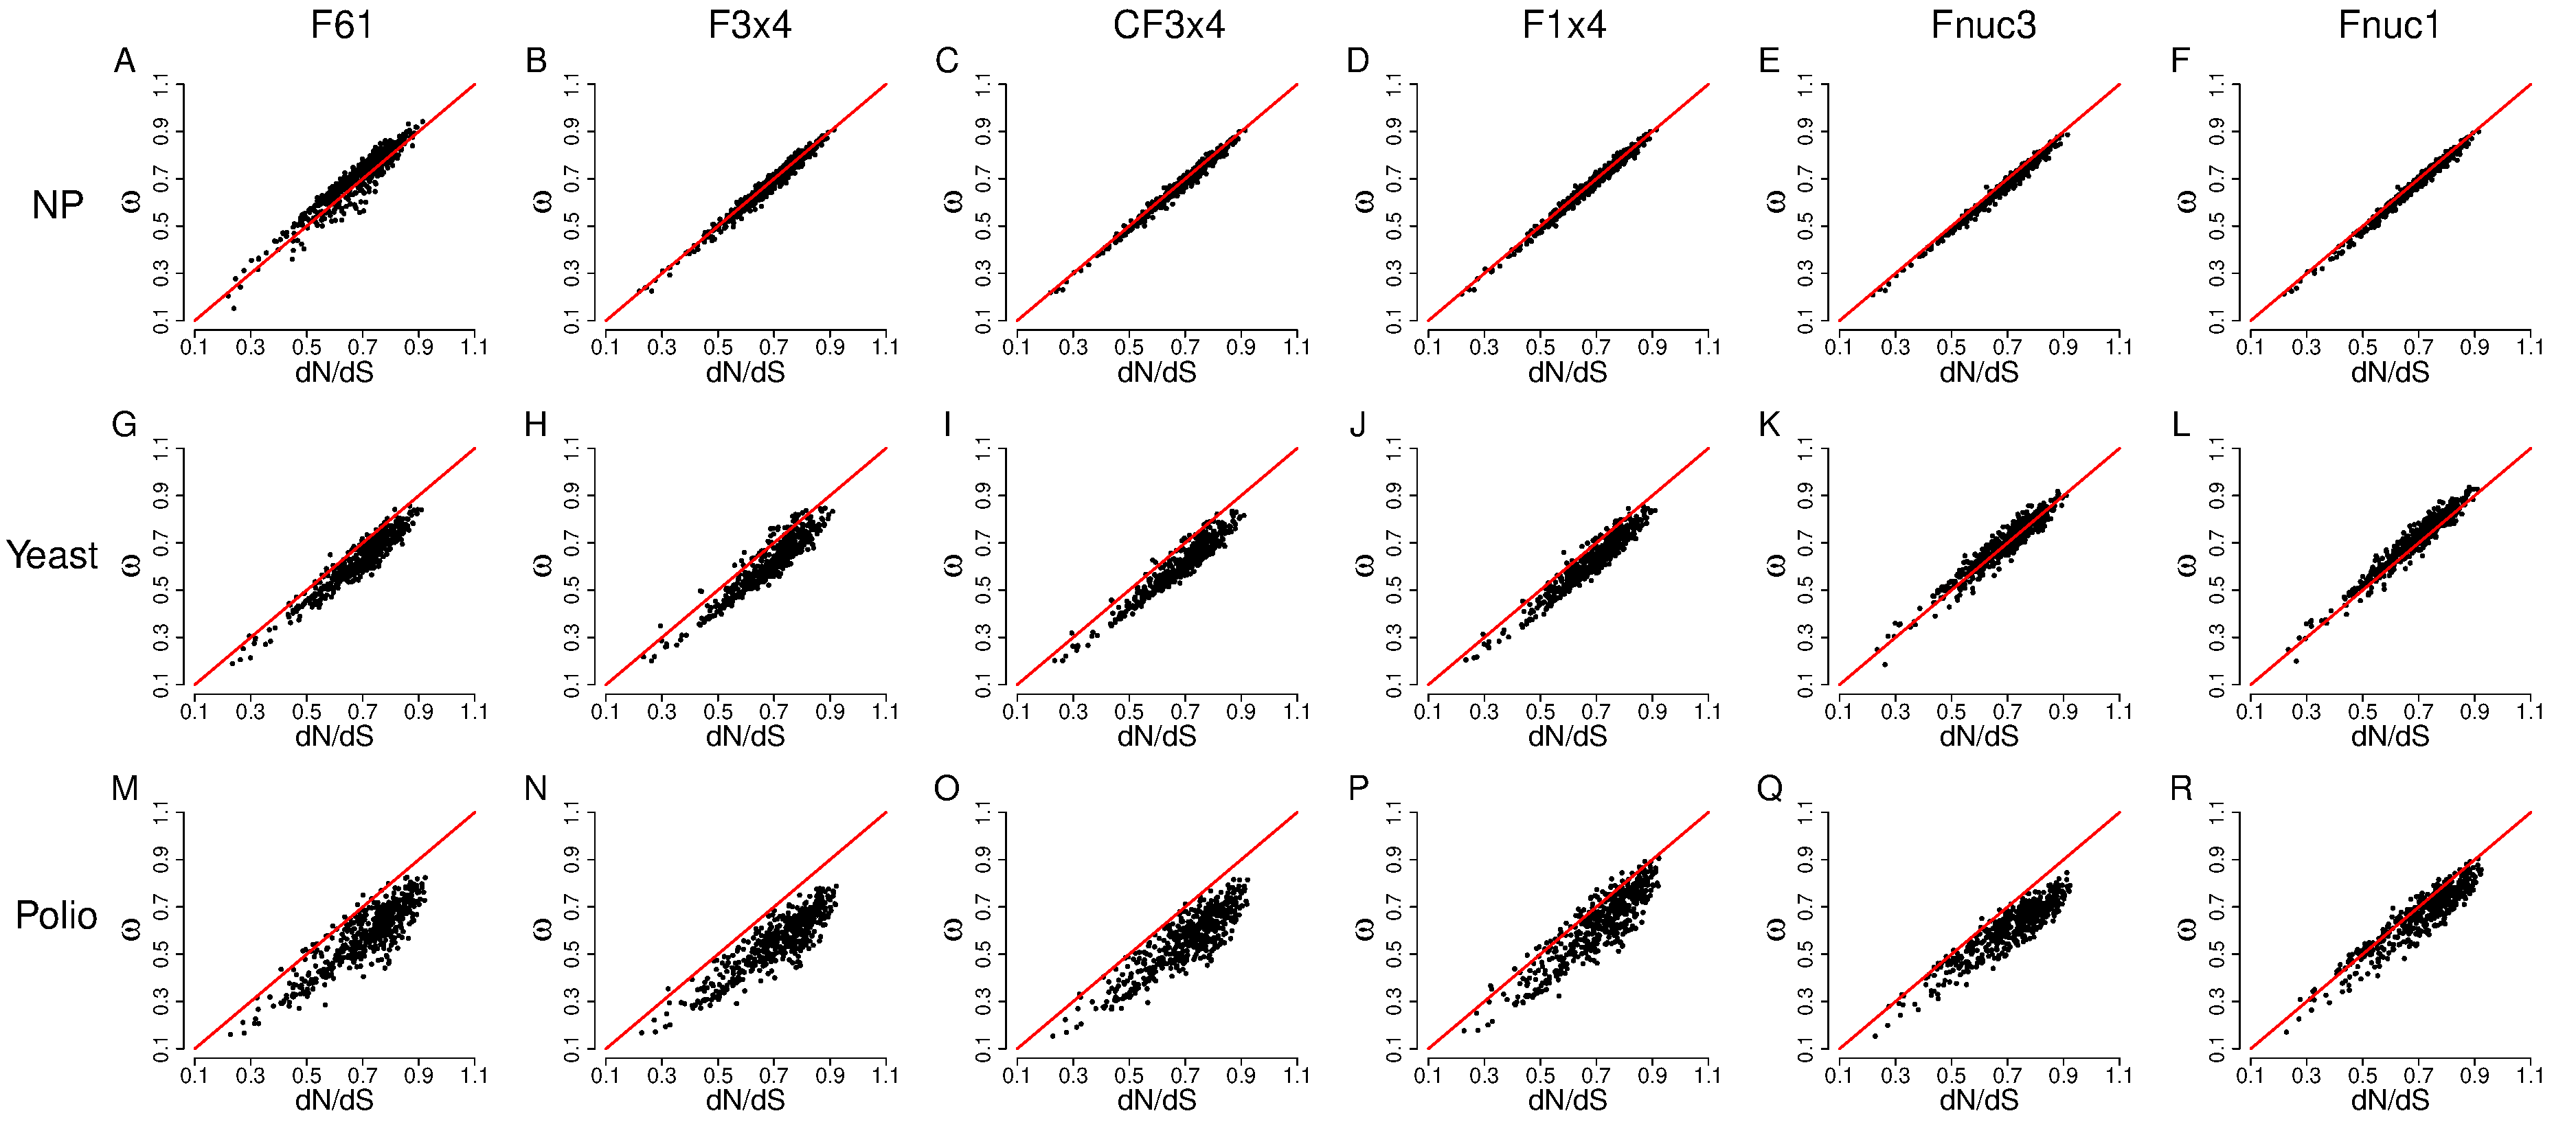
\includegraphics[width=9.5in]{figures/SI/nyp_regression.pdf}
	\vspace{0.5cm}
	
	\textbf{Figure S1.} Regressions of $\omega$ MLEs on the true $dN/dS$ values, as calculated from scaled selection coefficients, for datasets simulated using experimental fitnesses and mutation rates. Each point represents an alignment, and each red line is the $x=y$ line.
\end{landscape}


\newpage

\begin{thebibliography}{79}
\providecommand{\natexlab}[1]{#1}
\expandafter\ifx\csname urlstyle\endcsname\relax
  \providecommand{\doi}[1]{doi:\discretionary{}{}{}#1}\else
  \providecommand{\doi}{doi:\discretionary{}{}{}\begingroup
  \urlstyle{rm}\Url}\fi
  
\bibitem[{Burnham and Anderson(2004)}]{BurnhamAnderson2004}
Burnham K~P, Anderson D~R. 2004.
\newblock Multimodel inference: understanding {AIC} and {BIC} in model
  selection.
\newblock Sociol Method Res 33:261 -- 304.

\end{thebibliography}

\end{document}